\documentclass[12pt]{article}

% a template that a friend gave, it's worked well enough for me
% i have added some packages and stuff that have proved useful

\usepackage{fancyhdr}
\usepackage{tipa}
\usepackage{fontspec}
\usepackage{amsfonts}
\usepackage{enumitem}
\usepackage[margin=1in]{geometry}
\usepackage{graphicx}
\usepackage{float}
\usepackage{amsmath}
\usepackage{braket}
\usepackage{amssymb}
\usepackage{booktabs}
\usepackage{hyperref}
\usepackage{mathtools}
\usepackage{xcolor}
\usepackage{float}
\usepackage{algpseudocodex}
\usepackage{titlesec}
\usepackage{bbm}

\pagestyle{fancy}
\fancyhf{} % sets both header and footer to nothing
\lhead{Kevin Sheng}
\setmainfont{Comic Neue}
\renewcommand{\headrulewidth}{1pt}
\setlength{\headheight}{0.75in}
\setlength{\oddsidemargin}{0in}
\setlength{\evensidemargin}{0in}
\setlength{\voffset}{-.5in}
\setlength{\headsep}{10pt}
\setlength{\textwidth}{6.5in}
\setlength{\headwidth}{6.5in}
\setlength{\textheight}{8in}
\renewcommand{\headrulewidth}{0.5pt}
\renewcommand{\footrulewidth}{0.3pt}
\setlength{\textwidth}{6.5in}
\usepackage{setspace}
\usepackage{multicol}
\usepackage{float}
\setlength{\columnsep}{1cm}
\setlength\parindent{24pt}
\usepackage [english]{babel}
\usepackage [autostyle, english = american]{csquotes}
\MakeOuterQuote{"}

\setlength{\parskip}{6pt}
\setlength{\parindent}{0pt}

\titlespacing\section{0pt}{12pt plus 4pt minus 2pt}{0pt plus 2pt minus 2pt}
\titlespacing\subsection{0pt}{12pt plus 4pt minus 2pt}{0pt plus 2pt minus 2pt}
\titlespacing\subsubsection{0pt}{12pt plus 4pt minus 2pt}{0pt plus 2pt minus 2pt}

\hypersetup{colorlinks=true, urlcolor=blue}

\newcommand{\correction}[1]{\textcolor{red}{#1}}


\rhead{Math 180}

\makeatletter
\def\@seccntformat#1{%
  \expandafter\ifx\csname c@#1\endcsname\c@section\else
  \csname the#1\endcsname\quad
  \fi}
\makeatother

\begin{document}

\section{Chapter 5.3}

\begin{enumerate}
    \item[3] \begin{enumerate}
            \item I'll prove by innduction that for any $(u, v) \in E$, there exists
                  a Hamiltonian \textit{path} starting at $u$ and ending at $v$.
                  This extends to a cycle, since $u$ and $v$ are linked.

                  The base case, $n=3$, is trivial, since $T^{(3)}$ in that case is just a triangle.

                  For the inductive step, consider any edgee $(u, v)$.
                  $T$ is a tree, so removing this edge will give two smaller trees.

                  There's two cases we have to consider:
                  \begin{itemize}
                      \item If $u$ is a leaf, then we start our path at $u$ and jump
                            to any $v' \ne u$ that's connected to $v$ in $T$.
                            Such a $v'$ is guaranteed to exist because $|V| \ge 3$.
                            We can do this since the distance between $u$ and $v'$ is exactly $2$.

                            Since $(v, v') \in E$, by our inductive hypothesis we know
                            there exists a Hamiltonian path from $v'$ to $v$.
                            So our path from $u$ to $v$ can go like:
                            \[u, v', \text{hamiltonian from $v'$ to $v$}, v\]

                            This handles the case where $v$ is a leaf as well by symmetry.

                      \item OTOH, if there are nodes $u'$ and $v'$ connected to both $u$ and $v$ in $T$,
                            We do something similar:
                            \[u, \text{hamiltonian from $u$ to $u'$}, u', v', \text{hamiltonian from $v'$ to $v$}, v\]
                            We can go from $u'$ to $v'$ since they're $3$ apart.
                  \end{itemize}

            \item If we take any spanning tree $T$ of $G$ (which we can always do since $G$'s connected),
                  notice that $T^{(3)}$ is a subgraph of $G^{(3)}$ since any two nodes
                  that are at most $3$ away from each other in $T$ are definitely
                  at most $3$ apart in $G$ as well.

                  This allows us to take the Hamiltonian cycle in $T^{(3)}$
                  which we just proved exists and port it over to $G^{(3)}$. $\square$

            \item Consider the below graph $G$ and its corresopnding $G^{(2)}$:
                  \begin{center}
                      \hfill
                      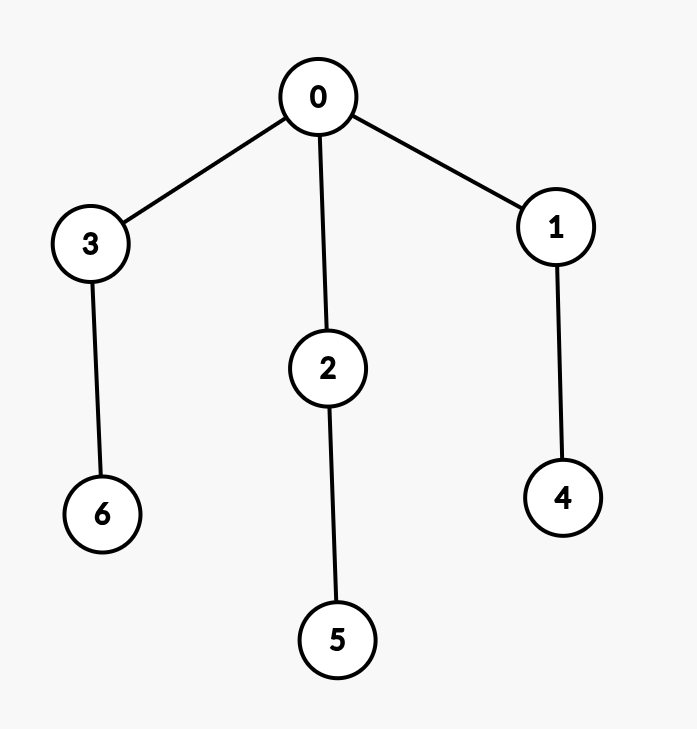
\includegraphics[width=5cm]{img/hw4/no_cycle}
                      \hfill
                      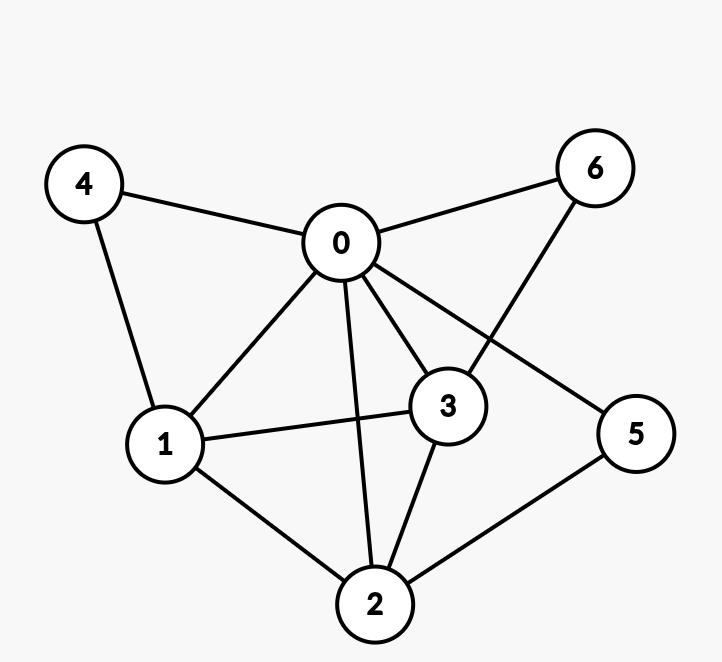
\includegraphics[width=5cm]{img/hw4/still_no_cycle}
                      \hfill \mbox{}
                  \end{center}
                  As you can see, there's no Hamiltonian cycle in this $G^{(2)}$.
        \end{enumerate}
\end{enumerate}

\pagebreak

\section{Chapter 5.4}

\begin{enumerate}
    \item[6] This follows by how we defined Kruskal's algorithm,
        which sorts the edges by weight.

        Since $w(e_1) < w(e_2) \iff w'(e_1) < w'(e_2)$,
        we know that if Kruskal's tries to process $e_1$ before $e_2$
        in the first version of the graph it'll do the same in the other graph.

    \item[8] Before we start, $d(x, y)$ be the Euclidean distance between points $x$ and $y$
        \begin{enumerate}
            \item BWOC say there existed an MST with a vertex $v$ of degree of at least $7$.
                  Ordering them in clockwise order, notice that since $\frac{360}{7} < 60^\circ$
                  there exists two vertices $u$ and $w$ s.t. connecting $(v, u)$ and $(v, w)$
                  in the plane has to be less than $60^\circ$.

                  From high school geometry we know that the side lengths of a triangle
                  can be ordered by how big the angles opposite them are.
                  $\theta < 60^\circ$ means the other two angles sum to something
                  greater than $120^\circ$ and that one of them must be at least
                  $60^\circ$ and $\theta$ by extension.

                  This then means that we can replace either $(v, u)$ or $(v, w)$ with $(u, w)$
                  which gives a strictly smaller spanning tree,
                  which is a contradiction. $\square$

            \item Consider any set of four points, as any two edges crossing
                  requires at least four points to exist.
                  Let these points be $A$, $B$, $C$, and $D$.
                  Say Kruskal's decided for some reason to add $AC$ and $BD$, two edges that cross.

                  Suppose the edges crossed at $E$ like so:
                  \begin{center}
                      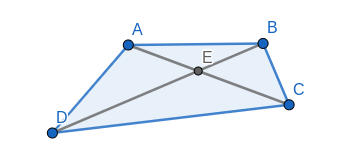
\includegraphics[width=6cm]{img/hw4/geo_wth}
                  \end{center}

                  Then we have
                  \begin{align*}
                      |AC|+|BD|
                       & = |AE|+|EC|+|BE|+|ED|     \\
                       & = (|AE|+|ED|)+(|EC|+|BE|) \\
                       & \ge |AD|+|BC|
                  \end{align*}
                  by the Triangle Inequality.
                  With a near-identical argument we can also conclude $|AC|+|BD| \ge |AB|+|DC|$.

                  Besides the two crossing edges, Kruskal's can't have added
                  more than one of the border edges since that would create a cycle.
                  This allows us to switch the crossing edges with a pair
                  of non-crossing, opposite-facing edges while not increasing the cost of the MST. $\square$
        \end{enumerate}

        \pagebreak

    \item[11] I'll just show that the greedy algorithm is a $\frac{3}{2}$-approximation
        algorithm since that implies being a $2$-approximation algorithm.

        Following the suggestions of the textbook hint, let
        the edges our greedy algorithm pick and the edges of a smallest edge cover be
        $\{e_1, \cdots, e_k\} $ and $\{\tilde{e}_1, \cdots, \tilde{e}_t\} $ respectively.

        Also, let $k_1 = |\{i : e_i \cap (e_1 \cup \cdots \cup c_{i-1}) = \varnothing\}|$
        and $t_1$ be something analagous but using $\tilde{e}_i$ instead.
        These represent the edges that cover two new vertices compared to one,
        since it's never optimal to pick an edge over two vertices that
        have already been covered.

        With that explanation above, $|V|=k+k_1=t+t_1$.
        By how we defined $k_1$, after selecting $k_1$ edges
        the greedy algorithm only picks edges that cover one new node.

        This means that every edge in what's counted by $t_1$
        has to have one node covered in what's counted by $k_1$,
        since the greedy algorithm would have picked that edge otherwise.

        Each edge has two points, so $k_1 \ge \frac{1}{2}t_1$ and $t_1-k_1 \le \frac{1}{2}t_1$ by extension.
        This gives us
        \begin{align*}
            k
             & = t+t_1-k_1                  \\
             & \le t+\frac{1}{2}t_1         \\
             & \le \frac{3}{2}t\quad\square
        \end{align*}
\end{enumerate}

\pagebreak

\section{Chapter 6.1}

\begin{enumerate}
    \item[1a] This is one of the platonic solids shown in the book:
        \begin{center}
            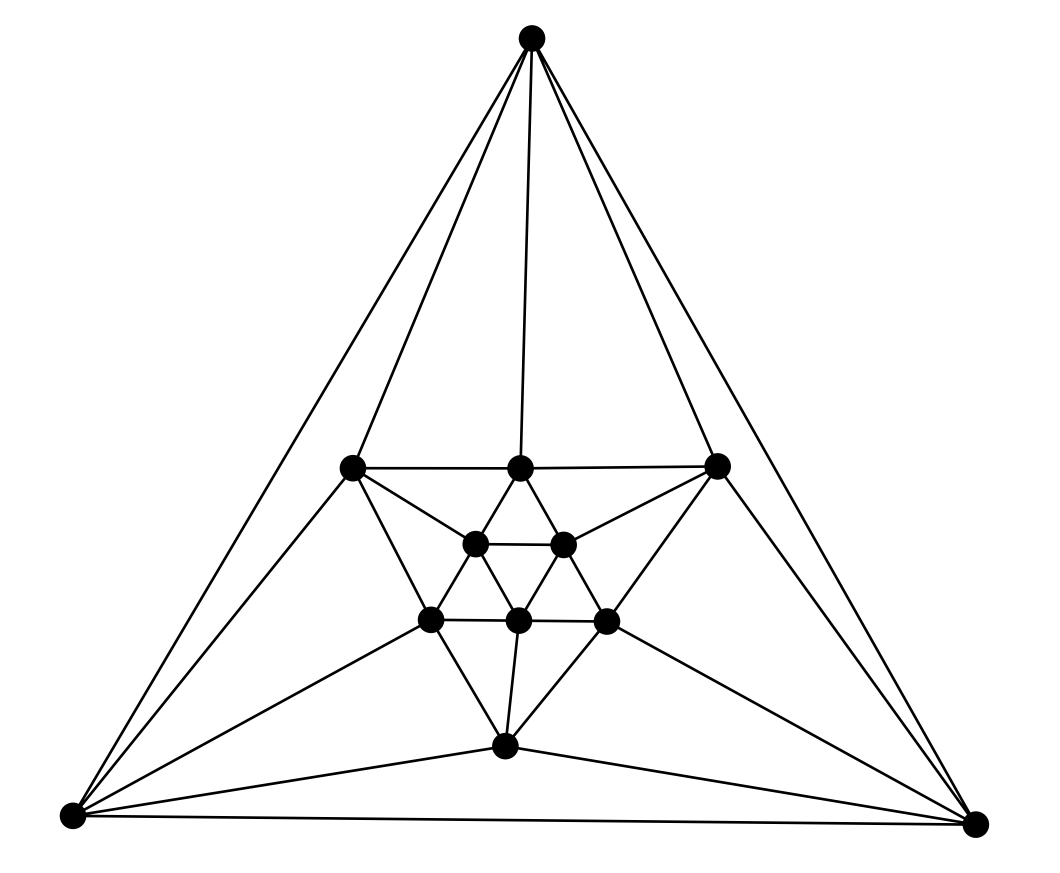
\includegraphics[width=8cm]{img/hw4/deg5_planar}
        \end{center}
        As you can see, it's planar, but all vertices have degree exactly $5$.

    \item[2b] We can draw the vertices on the top of the torus like so:
        \begin{center}
            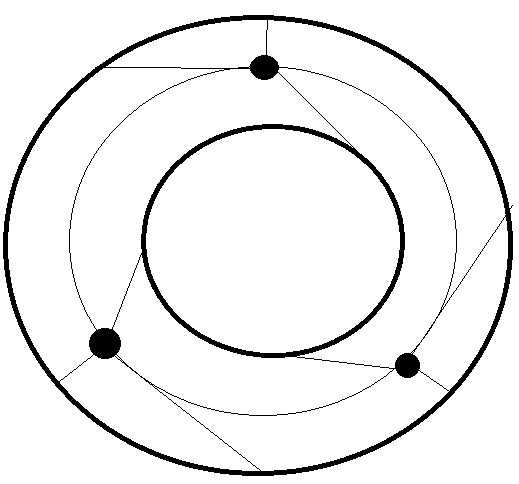
\includegraphics[width=7cm]{img/hw4/torus}
        \end{center}
        The bottom side looks basically the same as this as well.
\end{enumerate}

\pagebreak

\section{Chapter 6.3}

\begin{enumerate}
    \item[1] For all $n \in \mathbb{N}$, I'll construct a graph with $4n$ vertices and $8n-4$ edges.
        We construct this inductively.
        For $n=1$, a simple square suffices.
        It has $4$ edges, no triangles, and $4 = 2 \cdot 4 - 4$.

        For the inductive step, we "wrap" the current square in a larger square,
        adding $4$ new vertices and $8$ new edges like so:
        \begin{center}
            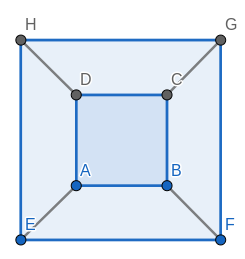
\includegraphics[width=6cm]{img/hw4/inductive_tri_free}
        \end{center}
        This increases the LHS by $8$ and the RHS by $2 \cdot 4 = 4$,
        so the equality is still satisfied. $\square$

    \item[7a] Since each dot can have at most $3$ lines coming into it,
        $3|V|-\sum_{i=1}^{n} \deg v_i \ge 0$.
        No edge is added at the start, so this quantity starts out at $3n$.

        When we add an edge, $|V|$ increases by $3$ and the degree summation increases by $4$,
        so the value of that expression decreases by $3$ with each move a player makes.

        After $3n-1$ moves, this quantity becomes $1$,
        meaning the graph can tolerate an increase of degree sum of at most $1$.
        No more moves can be made since we have to connect two dots first,
        and adding an edge increases the degree sum by $2$ each time. $\square$

        \pagebreak

    \item[7c] Notice that we can replace each cross with the following planar graph:
        \begin{center}
            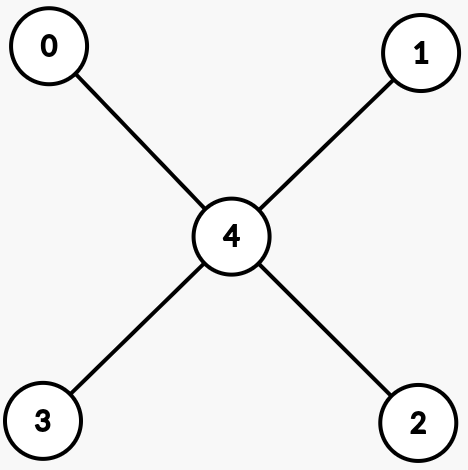
\includegraphics[width=5cm]{img/hw4/new_cross}
        \end{center}
        The end vertices are allowed to have degree at most $2$,
        while we just straight up aren't allowed to connect anything to the center.
        Define one of the end vertcies as "free" if it has degree $1$,
        i.e. it can take an incoming edge.

        Notice that when we connect two free ends and add
        a cross between them, it creates two more free ends.
        Thus, the number of free ends stays the same across all operations.

        The game ends only when all faces have only one free end in them.
        If there's a face with two or more free ends,
        we can connect them to keep on playing the game.

        Each operation does one of the two:
        \begin{itemize}
            \item Connect two components.
                  This doesn't create any new faces, so nothing changes.
                  We start with $n$ components, so this type can happen $n-1$ times.

            \item Create a new face by adding a cycle within an existing component.
                  This not only creates a new face, but it also splits the free
                  ends of the face among the two new faces.

                  There's $4n$ free ends, so we can split the set of free ends
                  into two smaller, nonempty sets at most $4n-1$ times.
        \end{itemize}
        $n-1+4n-1=\boxed{5n-2}$, so there's exactly $5n-2$ moves
        the playes can make before every face has only one free end
        and they run out of moves. $\square$
\end{enumerate}

\end{document}
